\documentclass[a4paper,12pt]{article} % This defines the style of your paper

\usepackage[top = 2.5cm, bottom = 2.5cm, left = 2.5cm, right = 2.5cm]{geometry} 

% Unfortunately, LaTeX has a hard time interpreting German Umlaute. The following two lines and packages should help. If it doesn't work for you please let me know.
\usepackage[T1]{fontenc}
\usepackage[utf8]{inputenc}
\usepackage{pifont}
% \usepackage{ctex}
\usepackage{amsthm, amsmath, amssymb, mathrsfs,mathtools}
\usepackage[ruled,vlined,linesnumbered]{algorithm2e}
% Defining a new theorem style without italics
\newtheoremstyle{nonitalic}% name
  {\topsep}% Space above
  {\topsep}% Space below
  {\upshape}% Body font
  {}% Indent amount
  {\bfseries}% Theorem head font
  {.}% Punctuation after theorem head
  {.5em}% Space after theorem head
  {}% Theorem head spec (can be left empty, meaning ‘normal’)
  
\theoremstyle{nonitalic}
\newtheorem{innercustomsol}{Solution}
\newenvironment{solution}[1]
  {\renewcommand\theinnercustomsol{#1}\innercustomsol}
  {\endinnercustomsol}

\newcounter{solutionctr}[section]
\renewcommand{\thesolutionctr}{(\alph{solutionctr})}

\newenvironment{autosolution}
  {\stepcounter{solutionctr}\begin{solution}{\thesolutionctr}}
  {\end{solution}}


\newtheorem{problem}{Problem}
\newtheorem{theorem}{Theorem}
\newtheorem{lemma}{Lemma}
\newtheorem{definition}{Definition}
\newtheorem{corollary}{Corollary}
\newtheorem{proposition}{Proposition}
% \newenvironment{proof}{{\noindent\it Proof}\quad}{\hfill $\square$\par}
\usepackage{color}

% The following two packages - multirow and booktabs - are needed to create nice looking tables.
\usepackage{multirow} % Multirow is for tables with multiple rows within one cell.
\usepackage{booktabs} % For even nicer tables.

% As we usually want to include some plots (.pdf files) we need a package for that.
\usepackage{graphicx} 
\usepackage{subfigure}


% The default setting of LaTeX is to indent new paragraphs. This is useful for articles. But not really nice for homework problem sets. The following command sets the indent to 0.
\usepackage{setspace}
\setlength{\parindent}{0in}
\usepackage{longtable}

% Package to place figures where you want them.
\usepackage{float}

% The fancyhdr package let's us create nice headers.
\usepackage{fancyhdr}

\usepackage{fancyvrb}

%Code environment 
\usepackage{listings} % Required for insertion of code
\usepackage{xcolor} % Required for custom colors

% Define colors for code listing
\definecolor{codegreen}{rgb}{0,0.6,0}
\definecolor{codegray}{rgb}{0.5,0.5,0.5}
\definecolor{codepurple}{rgb}{0.58,0,0.82}
\definecolor{backcolour}{rgb}{0.95,0.95,0.92}

% Code listing style named "mystyle"
\lstdefinestyle{mystyle}{
    backgroundcolor=\color{backcolour},   
    commentstyle=\color{codegreen},
    keywordstyle=\color{magenta},
    numberstyle=\tiny\color{codegray},
    stringstyle=\color{codepurple},
    basicstyle=\ttfamily\footnotesize, % Change to serif font
    breakatwhitespace=false,         
    breaklines=true,                 
    captionpos=b,                    
    keepspaces=true,                 
    numbers=left,                    
    numbersep=5pt,                  
    showspaces=false,                
    showstringspaces=false,
    showtabs=false,                  
    tabsize=2
}

\lstset{style=mystyle}

%%%%%%%%%%%%%%%%%%%%%%%%%%%%%%%%%%%%%%%%%%%%%%%%
% 3. Header (and Footer)
%%%%%%%%%%%%%%%%%%%%%%%%%%%%%%%%%%%%%%%%%%%%%%%%

% To make our document nice we want a header and number the pages in the footer.

\pagestyle{fancy} % With this command we can customize the header style.

\fancyhf{} % This makes sure we do not have other information in our header or footer.

\lhead{\footnotesize EI035 Econometrics I}% \lhead puts text in the top left corner. \footnotesize sets our font to a smaller size.

%\rhead works just like \lhead (you can also use \chead)
\rhead{\footnotesize Jingle Fu} %<---- Fill in your lastnames.

% Similar commands work for the footer (\lfoot, \cfoot and \rfoot).
% We want to put our page number in the center.
\cfoot{\footnotesize \thepage}
\IfFileExists{upquote.sty}{\usepackage{upquote}}{}
\begin{document}


\thispagestyle{empty} % This command disables the header on the first page. 

\begin{tabular}{p{15.5cm}} % This is a simple tabular environment to align your text nicely 
{\large \bf EI035 Econometrics I} \\
The Graduate Institute, Fall 2024, Marko Milkota\\
\hline % \hline produces horizontal lines.
\\
\end{tabular} % Our tabular environment ends here.

\vspace*{0.3cm} % Now we want to add some vertical space in between the line and our title.

\begin{center} % Everything within the center environment is centered.
	{\Large \bf PS5 Solutions} % <---- Don't forget to put in the right number
	\vspace{2mm}
	
        % YOUR NAMES GO HERE
	{\bf Jingle Fu} % <---- Fill in your names here!
		
\end{center}  

\vspace{0.4cm}
\setstretch{1.2}

\section*{Problem 1}

\begin{autosolution}
    \ 

    Yes, there are missing values in the data set.
    The initial number of observations is 99457,
    The dataset's reported missing values indicate that only 
    \textit{age} has missing observations (119 missing values). 
    After dropping these, we end up with 99338 observations.

    \begin{lstlisting}[language=R]
rm(list = ls())
library(tidyverse)
library(ggplot2)
library(dplyr)
library(broom)
library(stats)
library(stargazer)
library(car)

set.seed(2024)

dat <- read.csv("dat_SalesCustomers.csv")
variables_to_check <- c("category", "price", "gender", "age", "payment_method")
missing_counts <- sapply(dat[variables_to_check], function(x) sum(is.na(x)))
print("Number of missing values in each variable:")
print(missing_counts)

dat_clean <- dat[complete.cases(dat[variables_to_check]), ]

num_observations <- nrow(dat_clean)
print(paste("Number of observations after removing missing values:", num_observations))
    \end{lstlisting}
\end{autosolution}

\begin{autosolution}
    \

    Define
    \begin{align*}
        \text{paid\_in\_cash}_i &= \mathbf{1}\{\text{payment\_method}_i = \text{Cash}\} \\
        \text{male}_i &= \mathbf{1}\{\text{gender}_i = \text{Male}\}
    \end{align*}

    The fraction of transactions carried out in cash is
    \[
    \frac{1}{n}\sum_{i=1}^n \text{paid\_in\_cash}_i.
    \]
    Empirically, this is about $44.69\%$.

    The fraction of overall sales carried out in cash is
    \[
    \frac{\sum_{i=1}^n \text{paid\_in\_cash}_i \cdot price_i}{\sum_{i=1}^n price_i}.
    \]
    Empirically, this fraction is about $44.79\%$.

    These results indicate that cash payments represent nearly half of all transactions and sales value.

    \begin{lstlisting}[language=R]
dat_clean$paid_in_cash <- ifelse(dat_clean$payment_method == "Cash", 1, 0)
dat_clean$male <- ifelse(dat_clean$gender == "Male", 1, 0)
fraction_cash_transactions <- mean(dat_clean$paid_in_cash)
print(paste("Fraction of transactions carried out in cash:", 
            round(fraction_cash_transactions * 100, 2), "%"))

total_sales <- sum(dat_clean$price)
cash_sales <- sum(dat_clean$price[dat_clean$paid_in_cash == 1])
fraction_cash_sales <- cash_sales / total_sales
print(paste("Fraction of overall sales carried out in cash:", 
            round(fraction_cash_sales * 100, 2), "%"))
    \end{lstlisting}
\end{autosolution}

\begin{autosolution}
    \

    We now consider only the first $n=1000$ observations. Let the categories be divided into five mutually exclusive groups: 
    Clothes and Shoes (C), Cosmetics (Cos), Food (F), Technology (T), and Other (O). Define indicator variables:
    \begin{align*}
        d_{C,i} &= \mathbf{1}\{\text{category}_i=\text{Clothes and Shoes}\} \\
        d_{Cos,i} &= \mathbf{1}\{\text{category}_i=\text{Cosmetics}\} \\
        d_{F,i} &= \mathbf{1}\{\text{category}_i=\text{Food}\} \\
        d_{T,i} &= \mathbf{1}\{\text{category}_i=\text{Technology}\} \\
        d_{O,i} &= 1 - (d_{C,i}+d_{Cos,i}+d_{F,i}+d_{T,i}).
    \end{align*}
    The fraction of transactions in category $j$ is
    \[
    \frac{1}{1000}\sum_{i=1}^{1000} d_{j,i}.
    \]
    The fraction of sales in category $j$ is
    \[
    \frac{\sum_{i=1}^{1000} d_{j,i} \cdot price_i}{\sum_{i=1}^{1000} price_i}.
    \]
    Empirically:
    \begin{itemize}
        \item Transactions fraction: Clothes/Shoes: 43.8\%, Cosmetics: 14.8\%, Food: 14.0\%, Technology: 5.0\%, Other: 22.4\%.
        \item Sales fraction: Clothes/Shoes: 70.58\%, Cosmetics: 2.72\%, Food: 0.32\%, Technology: 23.9\%, Other: 2.49\%.
    \end{itemize}
    The result shows that most transactions and sales are in the Clothes/Shoes category. 
    Technology, though having the lowest transaction fraction, has the second-highest sales fraction, 
    meaning that it has the highest average price.

    \begin{lstlisting}[language=R]
dat_1000 <- dat_clean[1:1000, ]

dat_1000$clothes_shoes <- ifelse(dat_1000$category %in% c("Clothing", "Shoes"), 1, 0)
dat_1000$cosmetics <- ifelse(dat_1000$category == "Cosmetics", 1, 0)
dat_1000$food <- ifelse(dat_1000$category %in% c("Food", "Food & Beverage"), 1, 0)
dat_1000$technology <- ifelse(dat_1000$category == "Technology", 1, 0)

dat_1000$other_category <- ifelse(dat_1000$clothes_shoes + dat_1000$cosmetics + dat_1000$food + dat_1000$technology == 0, 1, 0)

all(dat_1000$clothes_shoes + dat_1000$cosmetics + dat_1000$food + dat_1000$technology + dat_1000$other_category == 1)

fraction_transactions <- c(
  "Clothes and Shoes" = mean(dat_1000$clothes_shoes),
  "Cosmetics" = mean(dat_1000$cosmetics),
  "Food" = mean(dat_1000$food),
  "Technology" = mean(dat_1000$technology),
  "Other" = mean(dat_1000$other_category)
)
print("Fraction of transactions in each category:")
print(round(fraction_transactions * 100, 2))

total_sales_1000 <- sum(dat_1000$price)
sales_clothes_shoes <- sum(dat_1000$price[dat_1000$clothes_shoes == 1])
sales_cosmetics <- sum(dat_1000$price[dat_1000$cosmetics == 1])
sales_food <- sum(dat_1000$price[dat_1000$food == 1])
sales_technology <- sum(dat_1000$price[dat_1000$technology == 1])
sales_other <- sum(dat_1000$price[dat_1000$other_category == 1])

fraction_sales <- c(
  "Clothes and Shoes" = sales_clothes_shoes / total_sales_1000,
  "Cosmetics" = sales_cosmetics / total_sales_1000,
  "Food" = sales_food / total_sales_1000,
  "Technology" = sales_technology / total_sales_1000,
  "Other" = sales_other / total_sales_1000
)

print("Fraction of sales in each category:")
print(round(fraction_sales * 100, 2))
    \end{lstlisting}
\end{autosolution}

\begin{autosolution}
    \
    
    To find the Maximum Likelihood Estimator (MLE) $\hat{\beta}$, we differentiate the log-likelihood with respect to $\beta$. Let $\phi(\cdot)$ denote the standard normal PDF. We use:
    \[
    \frac{d}{dt}\log(\Phi(t)) = \frac{\phi(t)}{\Phi(t)}, \quad \text{and} \quad \frac{d}{dt}\log(1-\Phi(t)) = -\frac{\phi(t)}{1-\Phi(t)}.
    \]
    For each element $\beta_j$ of $\beta$, the derivative of the log-likelihood is:
    \[
    \frac{\partial \ell(\beta;Z_n)}{\partial \beta_j} = \sum_{i=1}^n \left[y_i \frac{\phi(x_i'\beta)}{\Phi(x_i'\beta)} - (1-y_i)\frac{\phi(x_i'\beta)}{1-\Phi(x_i'\beta)}\right]x_{ij}.
    \]
    Stacking all partial derivatives together, the gradient (score vector) is:
    \[
    \nabla_{\beta}\ell(\beta;Z_n) = \sum_{i=1}^n \left[ \frac{y_i - \Phi(x_i'\beta)}{\Phi(x_i'\beta)(1-\Phi(x_i'\beta))} \phi(x_i'\beta) \right] x_i.
    \]
    Often written more simply as:
    \[
    \nabla_{\beta}\ell(\beta;Z_n) = \sum_{i=1}^n \left[ y_i \frac{\phi(x_i'\beta)}{\Phi(x_i'\beta)} - (1-y_i)\frac{\phi(x_i'\beta)}{1-\Phi(x_i'\beta)} \right] x_i.
    \]
    \underline{Step 1: Characterizing the MLE $\hat{\beta}$}
    
    The MLE $\hat{\beta}$ sets the gradient to zero:
    \[
    \nabla_{\beta}\ell(\hat{\beta};Z_n) = 0.
    \]
    Substituting back:
    \[
    \sum_{i=1}^n \left[ y_i \frac{\phi(x_i'\hat{\beta})}{\Phi(x_i'\hat{\beta})} - (1-y_i)\frac{\phi(x_i'\hat{\beta})}{1-\Phi(x_i'\hat{\beta})} \right] x_i = 0.
    \]
    This is a system of $k$ nonlinear equations in the $k$ unknowns $\hat{\beta} = (\hat{\beta}_1, \ldots, \hat{\beta}_k)'$.
    
    \underline{Step 2: No Closed-Form Solution}

    Unlike in linear regression or the logit model (even the logit doesn't have a closed form), the Probit model does not admit a closed-form solution for $\hat{\beta}$. The equation above must be solved using numerical optimization techniques such as the Newton-Raphson algorithm or other iterative methods.

    \underline{Step 3: Numerical Optimization}

    A common iterative procedure is:

    % \begin{note}[\textbf{Newton-Raphson Method}]
    %     \
    
    %     The Newton-Raphson method is a root-finding algorithm that uses the first few terms of the Taylor series of a function $f(x)$ in the vicinity of a starting point $x_0$ to find the root of the function. 
    %     The method is based on the idea that a continuous and differentiable function can be approximated by a straight line tangent to it. 
    %     The method is iterative and converges quadratically to the root.
    
        \begin{algorithm}[H]
            \caption{Newton-Raphson Method}
            \SetAlgoLined
            \SetKwInOut{Input}{Input}
            % \SetKwInOut{Output}{Output}
            
            \Input{Initialize $\beta_0$, tolerence level $\varepsilon>0$}
            % \Output{Decision to accept or reject $H_0$}
            
            \For{$m = 1$ \KwTo $M$}{
                Given $\beta ^m$, compute $\nabla_{\beta}\ell(\beta^{(m)};Z_n)$ and $[H(\beta^{(m)};Z_n)]$\;
                Set $    \beta^{(m+1)} = \beta^{(m)} - [H(\beta^{(m)};Z_n)]^{-1}\nabla_{\beta}\ell(\beta^{(m)};Z_n),$\;
                \eIf{$\left\| \beta^{m+1} - \beta^m  \right\| <\varepsilon $}{
                $\hat{\beta} = \beta^{m+1}$\;
                }{
                    Proceed to the next iteration\;
                }
            }
        \end{algorithm}
    % \end{note}
    where $H(\beta;Z_n)$ is the Hessian matrix of second derivatives evaluated at $\beta$. 
    Convergence is achieved when changes in $\beta$ or the norm of the gradient are below a given tolerance.

    The regression result is as follows:
    \[ 
    \begin{gathered}\hat{\beta}=
        \begin{bmatrix}
            \hat{\beta}_0\\
            \hat{\beta}_{price}\\
            \hat{\beta}_{male}\\
            \hat{\beta}_{age}\\
            \hat{\beta}_{cosmetics}\\
            \hat{\beta}_{food}\\
            \hat{\beta}_{technology}
        \end{bmatrix}
        =
        \begin{bmatrix}
            0.0682\\
            0.000112\\
            -0.0502\\
            -0.00183\\
            -0.2879\\
            -0.1195\\
            0.0640\\
            -0.4195
        \end{bmatrix}.
    \end{gathered}
    \]

    \textbf{Interpretation:}

    \begin{itemize}
        \item The coefficient on price is positive but very small, suggesting a tiny positive association
        of price with the probability of cash payment (not statistically significant).
        \item male is negative, but not significant, suggesting no strong gender effect on the
        probability of cash usage.
        \item age coefficient is negative and small, not statistically significant either.
        \item Some category dummies (like Clothes/Shoes) are significantly different from zero,
              indicating that the reference category (likely "Other") differs in payment method probability.            
    \end{itemize}
    \begin{table}[htbp!]

\caption{Simulation Summary Statistics for Question (d)}
\centering
\begin{tabular}[t]{lllrrr}
\toprule
  & Scenario & Regression & Mean & SD & Bias\\
\midrule
% Reg1 & Original DGP & Reg1 & -18.044602 & 2.7799242 & -23.0446020\\
% Reg2 & Original DGP & Reg2 & 4.756957 & 1.2464278 & -0.2430431\\
% Reg3 & Original DGP & Reg3 & 5.003735 & 0.1078386 & 0.0037353\\
Reg11 & $x_i|r_i=1 = x_i|r_i = 0$ & Reg1 & 5.530295 & 4.3563060 & 0.5302951\\
Reg21 & $x_i|r_i=1 = x_i|r_i = 0$ & Reg2 & 4.994777 & 1.3270007 & -0.0052234\\
Reg31 & $x_i|r_i=1 = x_i|r_i = 0$ & Reg3 & 4.991522 & 0.1105130 & -0.0084783\\
Reg12 &  $\beta_2=0$ & Reg1 & 5.211875 & 0.9578191 & 0.2118745\\
Reg22 &  $\beta_2=0$ & Reg2 & 5.282412 & 1.2969897 & 0.2824116\\
Reg32 &  $\beta_2=0$ & Reg3 & 5.005810 & 0.0950364 & 0.0058101\\
Reg13 &  $p(r_i=1)=0.1$ & Reg1 & -4.152274 & 2.6530512 & -9.1522744\\
Reg23 &  $p(r_i=1)=0.1$ & Reg2 & 4.941895 & 1.1553780 & -0.0581046\\
Reg33 &  $p(r_i=1)=0.1$ & Reg3 & 4.993826 & 0.0973356 & -0.0061737\\
Reg14 &  $\beta_3=50$ & Reg1 & -18.371055 & 6.5915167 & -23.3710551\\
Reg24 &  $\beta_3=50$ & Reg2 & 4.394012 & 6.1969404 & -0.6059882\\
Reg34 &  $\beta_3=50$ & Reg3 & 4.996611 & 0.1112587 & -0.0033893\\
\bottomrule
\end{tabular}
\end{table}
%% Table saved to d.tex


    \begin{lstlisting}[language=R]
X <- as.matrix(cbind(1, dat_1000[, c("price", "male", "age", "clothes_shoes", "cosmetics", "food", "technology")]))
y <- dat_1000$paid_in_cash

neg_log_likelihood <- function(beta, X, y) {
  X_beta <- X %*% beta
  log_phi_Xb <- pnorm(X_beta, log.p = TRUE)
  log_phi_minus_Xb <- pnorm(-X_beta, log.p = TRUE)
  ll <- sum(y * log_phi_Xb + (1 - y) * log_phi_minus_Xb)
  return(-ll)
}

neg_log_likelihood_grad <- function(beta, X, y) {
  X_beta <- X %*% beta
  phi_Xb <- dnorm(X_beta)
  Phi_Xb <- pnorm(X_beta)
  Phi_minus_Xb <- pnorm(-X_beta)
  epsilon <- 1e-16
  Phi_Xb <- pmax(Phi_Xb, epsilon)
  Phi_minus_Xb <- pmax(Phi_minus_Xb, epsilon)
  gradient <- -t(X) %*% ((y * phi_Xb / Phi_Xb) - ((1 - y) * phi_Xb / Phi_minus_Xb))
  return(as.vector(gradient))
}

initial_beta <- rep(0, ncol(X))

result <- optim(par = initial_beta, fn = neg_log_likelihood, gr = neg_log_likelihood_grad, X = X, y = y, method = "BFGS")

if (result$convergence == 0) {
  cat("Optimization converged.\n")
} else {
  cat("Optimization did not converge.\n")
}

beta_hat <- result$par
print("Estimated coefficients (beta_hat):")
print(beta_hat)

### Programming Method
model <- glm(paid_in_cash ~ price + male + age + clothes_shoes + cosmetics + food + technology, 
     data = dat_1000, family = binomial(link = "probit"))
stargazer(model, type = "latex", title = "Optimization model", out = "d.tex")

beta_hat2 <- coef(model)
print("Estimated coefficients (beta_hat):")
print(beta_hat2)
    \end{lstlisting}
\end{autosolution}

\begin{autosolution}
    \

    We define
    \[
    \gamma_1(\beta) = \Phi(x_2^{\prime} \beta) - \Phi(x_1^{\prime} \beta),
    \]
    where $x_1^{\prime} $ is a vector for a 30-year-old male buying Clothes/Shoes for 500 TRY, 
    and $x_2^{\prime}$ is the same vector but with age increased to 60 years old. 
    Only the age element of $x_i$ changes from 30 to 60.

    For our estimated $\hat{\beta}$,
    \[
    \gamma_1(\hat{\beta}) \approx -0.02096.
    \]
    This suggests that increasing age from 30 to 60 reduces the probability of cash payment by about 2.1 percentage points for this specific profile.

    For $\gamma_2(\beta)$, we do not condition on category. We take a weighted average of the partial effects across the five categories, with weights given by their share in total sales:
    \[
    \gamma_2(\hat{\beta}) = \sum_{j} w_j \left[\Phi(x_{2,j}^{\prime} \beta) - \Phi(x_{1,j}^{\prime} \beta)\right],
    \]
    where $w_j$ is the sales fraction for category $j$.

    Empirically,
    \[
    \gamma_2(\hat{\beta}) \approx -0.02077,
    \]
    very close to $\gamma_1(\hat{\beta})$, indicating a similar overall effect once categories are averaged by their sales importance.

    \begin{lstlisting}[language=R]
x_age_30 <- c(1, 500, 1, 30, 1, 0, 0, 0)

x_age_60 <- x_age_30
x_age_60[4] <- 60  # Update age to 35

prob_age_30 <- pnorm(sum(x_age_30 * beta_hat))
prob_age_60 <- pnorm(sum(x_age_60 * beta_hat))

gamma_1 <- prob_age_60 - prob_age_30
print(paste("Gamma_1 (effect of age increasing by 5 years):", gamma_1))

gamma_c <- numeric(length(fraction_sales))
names(gamma_c) <- names(fraction_sales)

for (cat in names(fraction_sales)) {
  clothes_shoes <- ifelse(cat == "Clothes and Shoes", 1, 0)
  cosmetics <- ifelse(cat == "Cosmetics", 1, 0)
  food <- ifelse(cat == "Food", 1, 0)
  technology <- ifelse(cat == "Technology", 1, 0)
  
  x_age_30_2 <- c(1, 500, 1, 30, clothes_shoes, cosmetics, food, technology)
  x_age_60_2 <- x_age_30_2
  x_age_60_2[4] <- 60  # Update age to 35
  
  prob_age_30_2 <- pnorm(sum(x_age_30_2 * beta_hat))
  prob_age_60_2 <- pnorm(sum(x_age_60_2 * beta_hat))
  
  gamma_c[cat] <- prob_age_60_2 - prob_age_30_2
}

gamma_2 <- sum(fraction_sales * gamma_c)
print(paste("Gamma_2 (weighted effect over categories):", gamma_2))        
    \end{lstlisting}
\end{autosolution}

\begin{autosolution}
    \ 

    Consider the linear model
    \[
    y_i = x_i' \beta + u_i
    \]
    where $ u_i \mid x_i \sim N(0,1) $.

    \underline{Step 1: Define the Objective Function}

    Define $\mathcal{B} = \left\{ \beta\in \mathbb{R}: \left\| \beta\right\| \leq c \right\}$ for some very large $c$. 
    
    The objective function is given by:
    \[
    \hat{\beta} = \arg \underset{\beta \in \mathcal{B}}{\min}Q_n(\beta) = \arg \underset{\beta \in \mathcal{B}}{\min} \frac{1}{n} \sum_{i=1}^n (y_i - x_i' \beta)^2
    \]

    \underline{Step 2: Express the Limiting Behavior of the Objective Function}

    The expected form of the objective function $Q_n(\beta)$ is:
    \begin{align*}
        Q(\beta) &= E[(y_i - x_i' \beta)^2]\\
        &= E[(x_i' \beta_0 + u_i - x_i' \beta)^2]\\
        &= E[(x_i' (\beta_0 - \beta) + u_i)^2] \\
        &= E[(x_i' (\beta_0 - \beta))^2] + 2E[x_i' (\beta_0 - \beta) u_i] + E[u_i^2] \\
        &= E[(x_i' (\beta_0 - \beta))^2] + \sigma^2 \\
        &= (\beta_0 - \beta)' E[x_i x_i'] (\beta_0 - \beta) + 1
    \end{align*}
    since $E[u_i \mid x_i] = 0$ and $\sigma^2 = 1$.

    \underline{Step 3: Show Minimization of $Q(\beta)$ at $\beta_0$}

    As $E[x_i x_i^{\prime}]$ is positive definite, the function $Q(\beta)$ is minimized at $\beta_0$ because:
    \[
    (\beta_0 - \beta)' E[x_i x_i'] (\beta_0 - \beta) \geq 0
    \]
    which is zero if and only if $\beta = \beta_0$.

    \underline{Step 4: Prove Uniform Convergence of $Q_n(\beta)$ to $Q(\beta)$}

    It's obvious that $m(x_i, y_i, \beta) = (y_i - x_i^{\prime} \beta)^{2}$ satisfies the first three conditions of the Uniform Law of Large Numbers(ULLN).
    
    We then prove the fourth one:
    \begin{align*}
        E\left[\underset{\beta \in \mathcal{B} }{\sup} \left \| m(x_i, y_i, \beta) \right \|  \right] &\leq E\left[\left | y_i \right |^2  \right] 
        + \underset{\beta \in \mathcal{B}}{\sup} 2E\left[ \left|y_i\right|\left|x_i\right|\left\| \beta \right\| \right]
        + \underset{\beta \in \mathcal{B}}{\sup} E\left[ \left|x_i \right| ^2 \left \| \beta^2 \right \| \right] \\
        & < \infty
    \end{align*}

    By ULLN:
    \[
    Q_n(\beta) \overset{p}{\rightarrow} Q(\beta), n \to \infty
    \]

    \underline{Step 5: Demonstrate the Consistency of $\hat{\beta}_n$}

    According to extremum estimator theory, if $Q_n(\beta)$ converges uniformly to $Q(\beta)$ and $Q(\beta)$ has a unique global minimum at $\beta_0$, then:
    \[
    \hat{\beta}_n \stackrel{p}{\rightarrow} \beta_0
    \]

    \textbf{Consistency of Probit Estimator:}

    First, we define $f(w_i; \theta) = \Phi(x_i^{\prime} \beta)^{y_t} \Phi(-x_i^{\prime} \beta)^{1-y_t}$,
    then $\log f(w_i; \theta) = y_i \log \Phi(x_i^{\prime} \beta) + (1-y_i) \log \Phi(-x_i^{\prime} \beta)$.

    \underline{Step 1: Theorem of Consistency}

    \begin{theorem}
        If $Q_n(w_i; \theta)$ is a function of $w_i$ and $\theta$ such that:
        \begin{itemize}
            \item[(A)] Parameter space $\Theta \in \mathbb{R}^{k}$ is compact, $\theta_0 \in \Theta$;
            \item[(B)] $Q_n(w_i; \theta)$ is continuous in $\theta \in \Theta$ for all $w_i$.
            \item[(C)] $Q_{n} (\theta)$ converges in probability to $Q(\theta)$ uniformly in $\theta \in \Theta$, and $Q(\theta)$ has a unique global minimum at $\theta_0$.
        \end{itemize}
        Define $Q_n(\hat{\theta}_n) = \underset{\theta \in \Theta}{\max} Q_n(\theta)$.

        Then, $\hat{\theta}_n \stackrel{p}{\rightarrow} \theta_0$.
    \end{theorem}

    \begin{proof}[\underline{Proof for Theorem 1}]
        \ 

        Let $N$ be a neignbourhood in $\mathbb{R}^k$ containing $\theta_0$.
        Then $\overline{N} \cap \Theta$ is compact $\Rightarrow \underset{\theta \in \overline{N} \cap \Theta}{\max} Q(\theta)$ exists.
        
        Denote $\varepsilon = Q(\theta_0) - \underset{\theta \in \overline{N} \cap \Theta}{\max} Q(\theta)$.

        Define incident $A_n$ as: 
        \[
        A_n: \left| \frac{1}{n}Q_n(\theta) - Q(\theta)\right| < \frac{\varepsilon}{2}.
        \]
        This implies that:
        \[
        \begin{cases}
            Q(\hat{\theta}_n) > \frac{1}{n} Q_n(\hat{\theta}_n) - \frac{\varepsilon}{2} \\
            \frac{1}{n} Q_n(\hat{\theta}_n) > Q(\theta_0) - \frac{\varepsilon}{2}
        \end{cases}
        \]
        But, as $Q_N(\hat{\theta}_n) \geq Q_n(\theta_0)$,
        \[
        Q(\hat{\theta}_n) > Q(\theta_0) - \varepsilon \Rightarrow \hat{\theta}_n \in N.
        \]
        Thus, $\mathbb{P}[A_n] \leq \mathbb{P}[\hat{\theta}_n \in N]$. Since we have $\underset{n\to \infty}{\lim}\mathbb{P}[A_n] = 1$ by (C),
        we have $\mathbb{P}[\hat{\theta}_n \in N] \to 1$.
        
        Hence $\hat{\theta}_n \stackrel{p}{\rightarrow} \theta_0$.
    \end{proof}
    In our cese, we take the parameter space $\mathcal{B} = \left\{ \beta \in \mathbb{R}^k: \left\| \beta \right\| < c \right\}$ for some large c,
    then, we have our compact parameter space $\Theta $, (A) is satisfied.

    As we take $Q_n(\theta) = \frac{1}{n}\ell(\beta; Z_n) = \frac{1}{n} \sum_{i=1}^{n} \log f(w_i; \beta)$,
    it's continuous in $\theta$ for all $w_i$, (B) is satisfied.

    So, we need to prove two conditions for the theorem to hold:
    \begin{enumerate}
        \item $Q_{n} (\theta)$ converges in probability to $Q(\theta)$ uniformly in $\theta \in \Theta$.
        \item (Identification) $Q(\theta)$ has a unique global minimum at $\theta_0$.
    \end{enumerate}

    \underline{Step 2: Identification of Probit Model}

    \begin{definition}[Identification]
        The information matrix $I(\theta)$ is defined as:
        \[
        I(\theta) = E\left[ \frac{\partial \ell^2(w_i; \theta)}{\partial \theta \partial \theta'}\right].
        \]
        If $I(\theta)$ is positive definite, then $\theta$ is identified.

        If $\theta$ is identified, it means that if $\theta \neq \theta_0$, then $f(w_i; \theta) \neq f(w_i; \theta_0)$.
    \end{definition}

    \begin{lemma}[Information Inequality]
        \
        
        If $\theta$ is identified, and $\mathbb{E}\left[\log f(w_i; \theta) < \infty\right]$ for all $\theta$,
        then $Q(\theta) = \mathbb{E}\left[ \vert \log f(w_i; \theta) \vert  \right]$ has a unique maximum at $\theta_0$.
    \end{lemma}

    \begin{proof}[\underline{Proof for Lemma 1}]
        For a random variable $Y$, by Jensen's inequality, we have:
        \[-\log \mathbb{E}[Y] < \mathbb{E}\left[-\log Y \right].\]

        In our case, we define a new random variable for $\theta \neq \theta_0$:
        \[
        Y = \frac{f(w_i; \theta)}{\mathbb{E}[f(w_i; \theta_0)]}.
        \]
        Then, we have:
        \begin{align*}
            Q(\theta_0) - Q(\theta) &= \mathbb{E}\left[ -\log Y \right] > -\log \mathbb{E}[Y] \\
                &= -\log \int f(w_i; \theta) d \theta = 0
        \end{align*}
    \end{proof}

    \underline{Step 3: Prove uniform convergence of Probit Model}

    To prove the uniform convergence of the Probit model, we give the second theorem:

    \begin{theorem}[Uniform Law of Large Numbers]
        \

        If $x_i$(or say, data) are i.i.d, and $\log f(w_i; \theta)$ is a function of $x_i, y_i, \theta$ such that:
        \begin{itemize}
            \item[(a)] Parameter space $\Theta \in \mathbb{R}^{k}$ is compact, $\theta_0 \in \Theta$;
            \item[(b)] $m(w_i; \theta)$ is continuous at each $\theta \in \Theta$ with probability to 1;
            \item[(c)] There exist a dominant function $d(w_i)$ such that $\left\| \log f(w_i; \theta) \right\| \leq \left\| d(w_i) \right\|$ $\forall \theta \in \Theta$;
            \item[(d)] $E\left[ d(w_i) \right] < \infty$.
        \end{itemize}
        then, $\mathbb{E}\left[\log f(w_i; \theta)\right]$ is continuous and
        \[
        \underset{\theta \in \Theta}{\sup} \left\| \frac{1}{n} \sum_{i=1}^{n} \log f(w_i; \theta) - \mathbb{E}\left[\log f(w_i; \theta)\right] \right\| \stackrel{p}{\rightarrow} 0.
        \]   
    \end{theorem}

    \begin{proof}[\underline{Proof for Theorem 2}]
        \
        
        For $\forall \theta_0 \in \Theta$, we define $\mathcal{B} (\theta_0, \delta) = \left\{ \theta \in \Theta: \left\| \theta - \theta_0 \right\| < \delta \right\}$
        and
        \[
        \Delta_{\delta}(w_i; \theta) = \underset{\theta \in \mathcal{B}(\theta_0, \delta)}{\sup} \left( \log f(w_i; \theta) - \mathbb{E}\left[\log f(w_i; \theta)\right] \right).
        \]
        For $\theta_0 \in \Theta$, we have:
        \[
        \mathbb{E}\left[\Delta_{\delta}(w_i; \theta) \to 0 \right] \text{ as } \delta \to 0.
        \]
        because
        \begin{enumerate}
            \item $\Delta_{\delta}(w_i; \theta_0) \to \log f(w_i; \theta) - \mathbb{E}\left[\log f(w_i; \theta)\right] $
            almost surely as $\delta \to 0$, because:
            \[
            \mathbb{P}\left[ \underset{\delta \to 0}{\lim} \underset{\theta \in \mathcal{B}(\theta_0, \delta)}{\sup} \log f(w_i; \theta) = \log f(w_i; \theta_0) \right] = 1
            \]
            by condition (b) and that $\mathbb{E}\left[\log f(w_i; \theta)\right]$ is continuous at $\theta_0$.
            \item By condition (c) and (d), we have:
            \[\Delta_{\delta}(w_i; \theta_0) \leq 2 \underset{\theta \in \mathcal{B}(\theta_0, \delta)}{\sup} \vert \log f(w_i; \theta) \vert \leq 2 d(w_i) \]
        \end{enumerate}
        So, for all $\theta \in \Theta$, $\varepsilon > 0$, $\exists \delta_{\varepsilon}(\theta)$, such that
        \[
        \mathbb{E}\left[\Delta_{\delta_{\varepsilon}(\theta)}(w_i; \theta) \right] < \varepsilon.
        \]
        Obviously, we can cover the entire parameter space with a finite number of $\mathcal{B} (\theta, \delta_{\varepsilon}(\theta)): \theta \in \Theta $, which is:
        \[
        \mathcal{B} \left(\theta_k, \delta_{\varepsilon}(\theta_k): k=1, 2, \cdots, K\right) \text{ s.t. } \Theta = \bigcup_{k=1}^{K} \mathcal{B} \left(\theta_k, \delta_{\varepsilon}(\theta_k)\right).
        \]
        Note that:
        \begin{align*}
        & \quad \underset{\theta \in \Theta}{\sup} \left[ \frac{1}{n} \sum_{i=1}^{n} \log f(w_i; \theta) - \mathbb{E}\left[\log f(w_i; \theta)\right] \right] \\
            &= \underset{k}{\max} \underset{\theta \in \mathcal{B}(\theta_k, \delta_{\varepsilon}(\theta_k))}{\sup} \left[ \frac{1}{n} \sum_{i=1}^{n} \log f(w_i; \theta) - \mathbb{E}\left[\log f(w_i; \theta)\right] \right] \\
            &\leq \underset{k}{\max} \frac{1}{n} \left[ \sum_{i=1}^{n} \underset{\theta \in \mathcal{B}(\theta_k, \delta_{\varepsilon}(\theta_k))}{\sup} \log f(w_i; \theta) - \mathbb{E}\left[\log f(w_i; \theta)\right] \right] \\
            &\leq \mathcal{O}_p(1) + \underset{k}{\max} \mathbb{E}^*\Delta_{\delta_{\varepsilon}(\theta_k)}(w_i; \theta_k) \\
            &= \mathcal{O}_p(1) + \varepsilon.
        \end{align*}
        where the second inequality holds by the Weak Law of Large Numbers (WLLN)
        because:
        \[
        \left| \underset{\theta \in \mathcal{B}(\theta_k, \delta_{\varepsilon}(\theta_k))}{\sup} \log f(w_i; \theta) \right| \leq d(w_i); \mathbb{E}[d(w_i)] < \infty.
        \]    
        and the third inequality holds by the definition of $\delta_{\varepsilon}(\theta_k)$.
        By analogous argument, we can prove that:
        \[ 
        \underset{\theta \in \Theta}{\inf} \left[ \frac{1}{n} \sum_{i=1}^{n} \log f(w_i; \theta) - \mathbb{E}\left[\log f(w_i; \theta)\right] \right] \geq O_p(1) - \varepsilon.
        \]
        Combing the two results, we have:
        \[
        \left| \frac{1}{n} \sum_{i=1}^{n}\log f(w_i; \theta) - \mathbb{E}[\log f(w_i; \theta)] \right| \to \mathcal{O}_p(1) = 0.
        \]
    \end{proof}
    Finishing the proof of Theorem 2, we can find that the Probit model still have to satisfy conditions (c) and (d) to hold the theorem.

    \underline{Step 4: Proof of Conditions (c) and (d) for ULLN}

    In this part, we show that identification and the uniform convergence of the Probit model are combined by
    the existence of $\mathbb{E}[x_i x_i^{\prime} ]$ and its nonsingularity.
    \begin{proof}[Proof for ULLN conditions (c) and (d)]
        \

        For this proof, we take two steps:

        \underline{Step 1: $\mathbb{E}\left[\left|\log f(w_i; \theta)\right|\right]$ is finite.}

        Let $\theta \neq \theta_0$, then 
        \begin{align*}
            \mathbb{E}\left[\left(x_i^{\prime} (\theta - \theta_0)\right)^2\right] &= (\theta - \theta_0)' \mathbb{E}[x_i x_i^{\prime}] (\theta - \theta_0) > 0 \\
            & \Rightarrow x_i^{\prime} (\theta - \theta_0) \neq 0 \\
            & \Rightarrow x_i^{\prime} \theta \neq x_i^{\prime} \theta_0 
        \end{align*}
        Since $\Phi$ is strictly monotone, this gives us $\Phi (x_i^{\prime} \theta) \neq \Phi(-x_i^{\prime} \theta)$.
        So that $f(w_i; \theta) = \Phi(x_i^{\prime} \beta)^{y_t} \Phi(-x_i^{\prime} \beta)^{1-y_t} \neq f(w_i; \theta_0)$.

        We know that $\frac{d \log \Phi(v)}{d x} = \frac{\phi(v)}{\Phi(v)}$ is convex and asymptotic to 0 as $v \to \infty$ and to $-v$ as $v \to -\infty$.

        We take the mean-value expansion around $\theta = 0$:
        \begin{align*}
            \left|\log \Phi(x_i^{\prime} \theta)\right| &= \left|\log \Phi(0) + \lambda(x_i^{\prime} \tilde{\theta}) x_i^{\prime} \theta \right| \\
            &\leq \left|\log \Phi(0)\right| + \left|\lambda(x_i^{\prime} \tilde{\theta}) x_i^{\prime} \theta\right| \\
            &\leq \left|\log \Phi(0)\right| + C\left(1 + \left|x_i^{\prime} \tilde{\theta}\right| \right) \left|x_i^{\prime} \theta\right| \\
            &\leq \left|\log \Phi(0)\right| + C\left(1 + \left\|x_i\right\| \left\| \theta \right\| \right) \left\|x_i\right\| \left\| \theta \right\|
        \end{align*}
        where $\lambda$ is the reverse Mills ratio.
        
        Since $1 - \Phi(v) = \Phi(-v)$ and $y$ are bounded, we have:
        \[
        \left|\log f(w_i; \theta)\right| \leq \left|\log \Phi(0)\right| + C\left(1 + \left\|x_i\right\| \left\| \theta \right\| \right) \left\|x_i\right\| \left\| \theta \right\|
        \]
        where $C$ is a constant.

        Thus, we could say that $\mathbb{E}\left[\left|\log f(w_i; \theta)\right|\right]$ is finite.

        \underline{Step 2: $\mathbb{E}[d(w_i)]$ exist, and is finite.}

        Based on Step 1, we could directly take
        \[d(w_i) = C\left(1 + \left\|x_i\right\|^2 \right).\]
        It's obvious that $\mathbb{E}[d(w_i)]$ is finite.
    \end{proof}

    Combining Lemma 1, Lemma 2, Theorem 1, and Theorem 2, we could say that the Probit model estimator is consistent.
\end{autosolution}

\begin{autosolution}
    \

    \begin{lstlisting}[language=R]
M <- 100
n <- nrow(dat_1000)
beta_age_bootstrap <- numeric(M)
gamma_1_bootstrap <- numeric(M)
gamma_2_bootstrap <- numeric(M)
set.seed(2024)

for (m in 1:M) {
  indices <- sample(1:n, size = n, replace = TRUE)
  dat_bootstrap <- dat_1000[indices, ]
  
  model_boot <- glm(paid_in_cash ~ price + male + age + clothes_shoes + cosmetics + food + technology, data = dat_bootstrap, family = binomial(link = "probit"))
  beta_hat_boot <- coef(model_boot)
  
  beta_age_bootstrap[m] <- beta_hat_boot["age"]
  
  x_age_30 <- c(1, 500, 1, 30, 1, 0, 0, 0)
  x_age_60 <- x_age_30
  x_age_60[4] <- 60  # Update age to 35
  prob_age_30 <- pnorm(sum(x_age_30 * beta_hat_boot))
  prob_age_60 <- pnorm(sum(x_age_60 * beta_hat_boot))
  gamma_1_bootstrap[m] <- prob_age_60 - prob_age_30
  
  gamma_c <- numeric(length(fraction_sales))
  names(gamma_c) <- names(fraction_sales)
  
  for (cat in names(fraction_sales)) {
    clothes_shoes <- ifelse(cat == "Clothes and Shoes", 1, 0)
    cosmetics <- ifelse(cat == "Cosmetics", 1, 0)
    food <- ifelse(cat == "Food", 1, 0)
    technology <- ifelse(cat == "Technology", 1, 0)
    
    x_age_30_2 <- c(1, 500, 1, 30, clothes_shoes, cosmetics, food, technology)
    x_age_60_2 <- x_age_30
    x_age_60_2[4] <- 60  # Update age to 35
    
    prob_age_30_2 <- pnorm(sum(x_age_30_2 * beta_hat_boot))
    prob_age_60_2 <- pnorm(sum(x_age_60_2 * beta_hat_boot))
    gamma_c[cat] <- prob_age_60_2 - prob_age_30_2
  }
  
  gamma_2_bootstrap[m] <- sum(fraction_sales * gamma_c)
}

hist(beta_age_bootstrap, main = "Bootstrap Distribution of Coefficient on Age", xlab = "Coefficient on Age", breaks = 20)
hist(gamma_1_bootstrap, main = "Bootstrap Distribution of Gamma_1", xlab = "Gamma_1", breaks = 20)
hist(gamma_2_bootstrap, main = "Bootstrap Distribution of Gamma_2", xlab = "Gamma_2", breaks = 20)
    \end{lstlisting}

    \begin{figure}[!htbp]
        \centering
        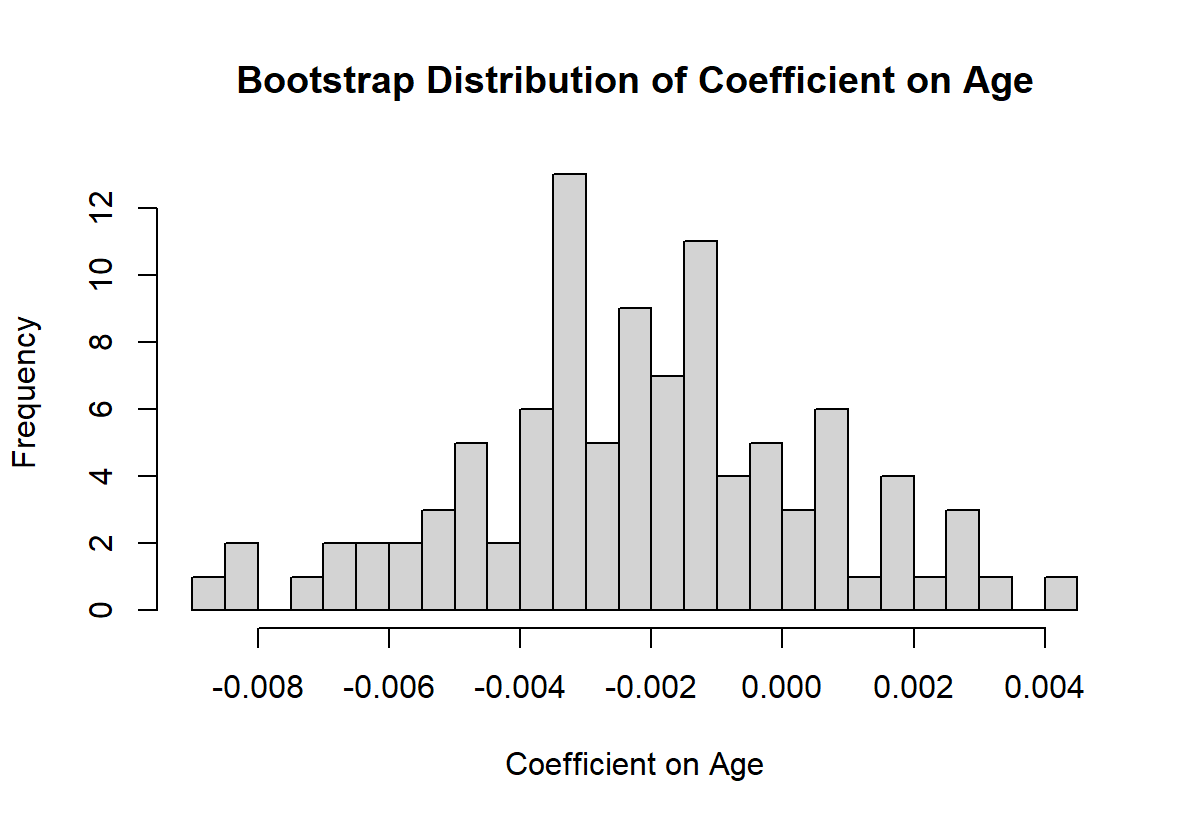
\includegraphics[width=0.5\linewidth]{g-1.png}
        \caption{Bootstrap Distribution of Coefficient on Age}
        \label{fig:g-1}

        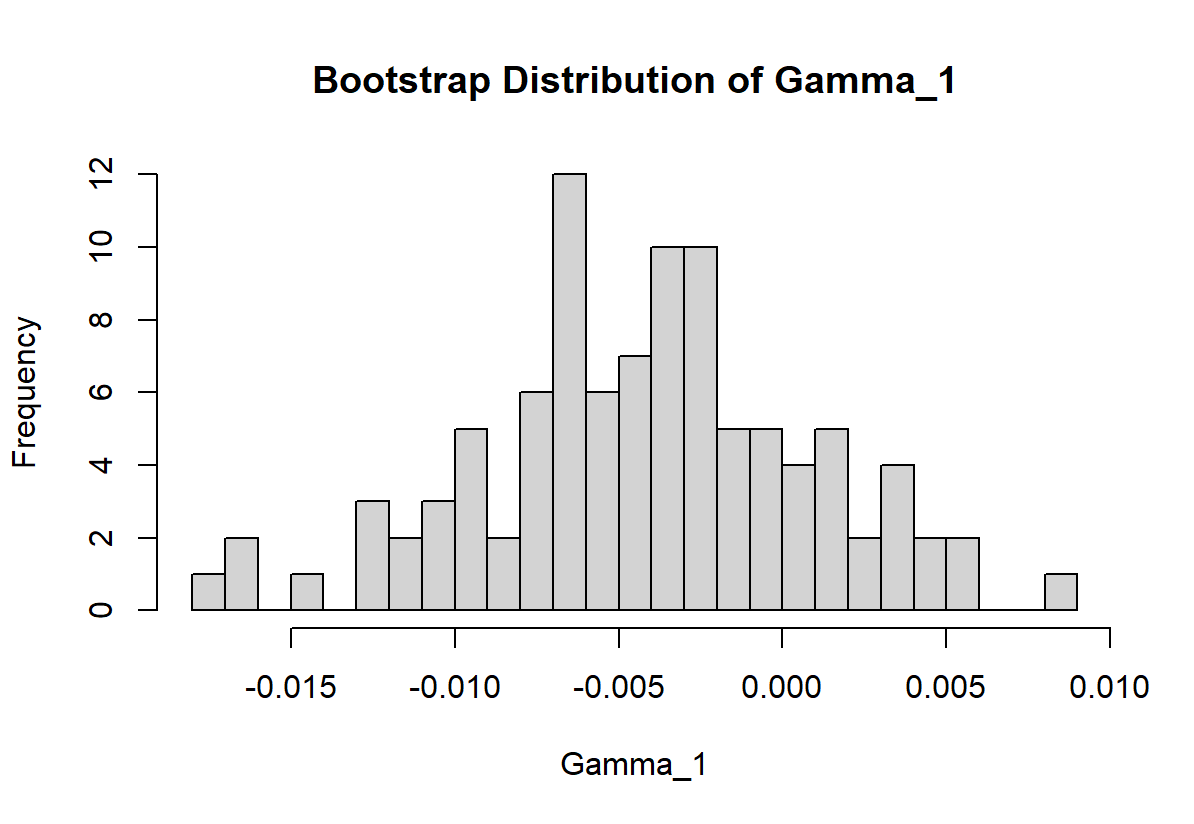
\includegraphics[width=0.5\linewidth]{g-2.png}
        \caption{Bootstrap Distribution of Gamma\_1}
        \label{fig:g-2}
        
        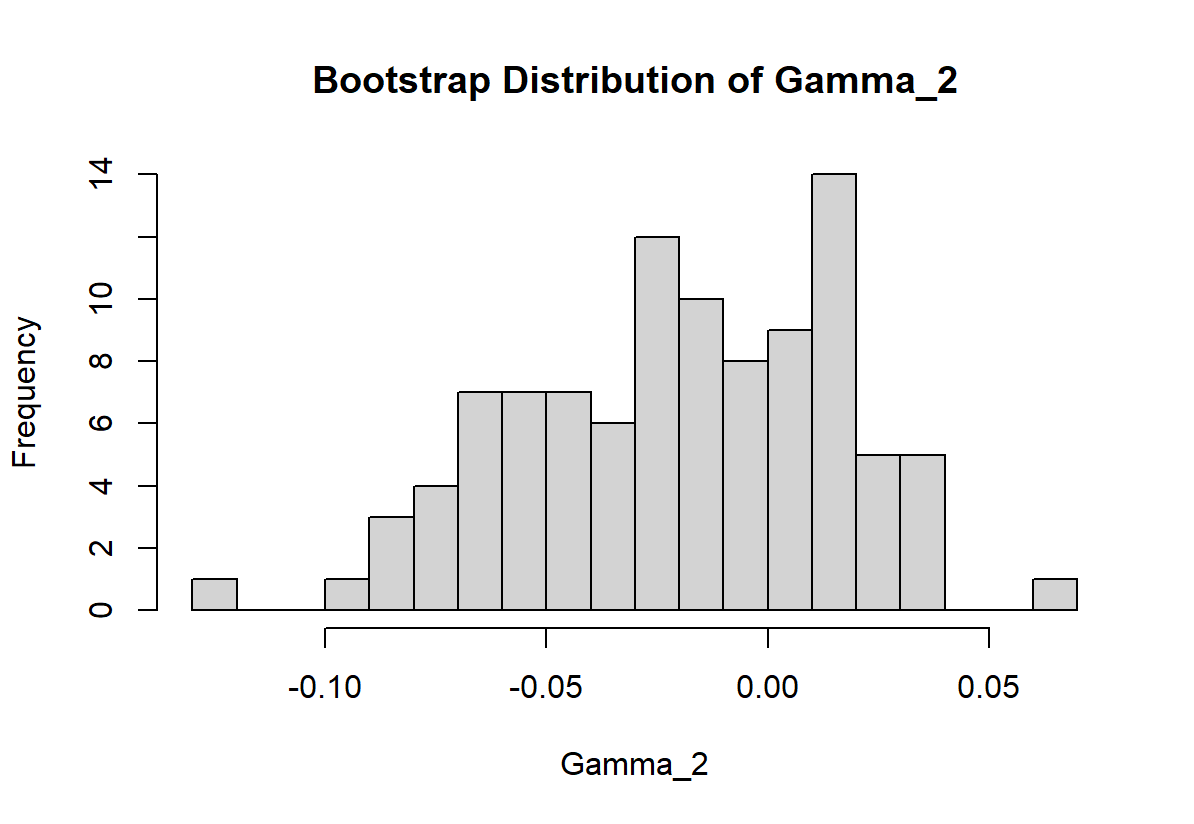
\includegraphics[width=0.5\linewidth]{g-3.png}
        \caption{Bootstrap Distribution of Gamma\_2}
        \label{fig:g-3}
    \end{figure}
\end{autosolution}

\pagebreak
\begin{autosolution}
    \

    For a sample $\{(y_i,x_i)\}_{i=1}^n$, the log-likelihood function is:
    \[
    \ell(\beta; Z_n) = \sum_{i=1}^n \left[ y_i \log(\Phi(x_i'\beta)) + (1 - y_i)\log(1 - \Phi(x_i'\beta)) \right].
    \]

    To derive the Hessian, focus on a single observation $i$ and then we will take expectations:
    \[
    \ell_i(\beta) = y_i \log(\Phi(t_i)) + (1 - y_i)\log(1 - \Phi(t_i)), \quad t_i = x_i'\beta.
    \]

    \underline{First Derivative (Score):}  

    First, take the derivative with respect to $t_i$:
    \[
    \frac{\partial \ell_i(\beta)}{\partial t_i} = y_i \frac{\phi(t_i)}{\Phi(t_i)} - (1 - y_i)\frac{\phi(t_i)}{1 - \Phi(t_i)},
    \]
    where $\phi(\cdot)$ is the standard normal PDF.

    Combine the fractions:
    \[
    \frac{\partial \ell_i(\beta)}{\partial t_i} 
    = \phi(t_i)\left[\frac{y_i}{\Phi(t_i)} - \frac{1 - y_i}{1 - \Phi(t_i)}\right].
    \]

    Find a common denominator $\Phi(t_i)(1-\Phi(t_i))$:
    \[
    \frac{\partial \ell_i(\beta)}{\partial t_i} 
    = \frac{\phi(t_i)}{\Phi(t_i)(1-\Phi(t_i))}(y_i - \Phi(t_i)).
    \]

    Since $y_i - \Phi(t_i) = y_i - p_i$, we have:
    \[
    \frac{\partial \ell_i(\beta)}{\partial t_i} = \frac{\phi(t_i)}{p_i(1-p_i)}(y_i - p_i).
    \]

    To get the gradient w.r.t. $\beta$, use chain rule:
    \[
    \frac{\partial \ell_i(\beta)}{\partial \beta} = \frac{\partial \ell_i(\beta)}{\partial t_i} x_i = \frac{\phi(t_i)}{p_i(1-p_i)}(y_i - p_i) x_i.
    \]

    This is the score vector for a single observation.

    \underline{Second Derivative (Hessian):}

    Now differentiate again with respect to $\beta$:
    \[
    \frac{\partial^2 \ell_i(\beta)}{\partial \beta \partial \beta'} = \frac{\partial}{\partial \beta}\left(\frac{\phi(t_i)}{p_i(1-p_i)}(y_i - p_i) x_i\right).
    \]

    Since $t_i = x_i'\beta$, $\frac{\partial t_i}{\partial \beta} = x_i$. Thus, second derivatives w.r.t. $\beta$ come through differentiating w.r.t. $t_i$, then applying chain rule again:
    \[
    \frac{\partial^2 \ell_i(\beta)}{\partial \beta \partial \beta'} = \left(\frac{\partial^2 \ell_i(\beta)}{\partial t_i^2}\right) x_i x_i'.
    \]

    So the main task is to find:
    \[
    \frac{\partial^2 \ell_i(\beta)}{\partial t_i^2}.
    \]

    We have:
    \[
    \frac{\partial \ell_i(\beta)}{\partial t_i} = \frac{\phi(t_i)}{p_i(1-p_i)}(y_i - p_i).
    \]

    Take the derivative w.r.t. $t_i$:
    \[
    \frac{\partial^2 \ell_i(\beta)}{\partial t_i^2} 
    = \frac{\partial}{\partial t_i}\left[\frac{\phi(t_i)}{p_i(1-p_i)}(y_i - p_i)\right].
    \]

    This involves the product rule and quotient rule. However, \textit{the key simplification occurs when we take expectations at the true parameter $\beta_0$}. Under the true model, $E[y_i]=p_i$, so $E[y_i - p_i]=0$. Terms involving $(y_i - p_i)$ vanish when taking expectation.

    At the true parameter, the Fisher information (which is $-E[\partial^2 \ell_i(\beta_0)/\partial \beta \partial \beta']$) simplifies dramatically. Instead of going through the full complex algebra of the second derivative in the $y_i$ form, we use the known result from standard Probit derivations:

    Under correct specification, the expected Hessian w.r.t. $t_i$ at $\beta_0$ is known to be:
    \[
    E\left[\frac{\partial^2 \ell_i(\beta_0)}{\partial t_i^2}\right] = -\frac{\phi(t_i)^2}{p_i(1-p_i)}.
    \]
    Thus:
    \[
    E\left[\frac{\partial^2 \ell_i(\beta_0)}{\partial \beta \partial \beta'}\right] 
    = E\left[\frac{\partial^2 \ell_i(\beta_0)}{\partial t_i^2} x_i x_i'\right] 
    = E\left[-\frac{\phi(t_i)^2}{p_i(1-p_i)} x_i x_i'\right].
    \]

    Multiplying by $-1$, the Fisher Information matrix (which is $H$ in the problem) is:
    \[
    H = E\left[\frac{\phi(x_i'\beta_0)^2}{\Phi(x_i'\beta_0)[1-\Phi(x_i'\beta_0)]} x_i x_i'\right].
    \]

    Since $1-\Phi(t_i)=\Phi(-t_i)$:
    \[
    H = E\left[\frac{\phi(x_i'\beta_0)^2}{\Phi(x_i'\beta_0)\Phi(-x_i'\beta_0)} x_i x_i'\right].
    \]

    In the dataset result, the given histograms for the bootstrap distributions and the asymptotic distributions show approximately symmetric, bell-shaped distributions. 
    This suggests that the normal approximation may be reasonable.

    \begin{figure}[!htbp]
        \centering
        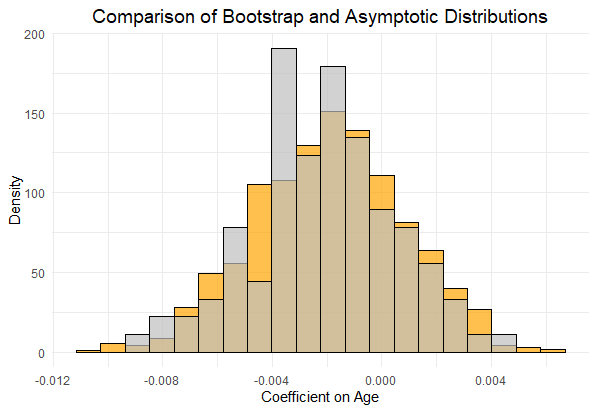
\includegraphics[width=0.5\linewidth]{h.png}
        \caption{Comparison of Bootstrap and Asymptotic Distributions}
        \label{fig:h}
    \end{figure}

    \begin{lstlisting}[language=R]
X <- as.matrix(cbind(1, dat_1000[, c("price", "male", "age", "clothes_shoes", "cosmetics", "food", "technology")]))
X_beta_hat <- X %*% beta_hat

log_phi_Xb <- dnorm(X_beta_hat, log = TRUE)
log_Phi_Xb <- pnorm(X_beta_hat, log.p = TRUE)

log_Phi_minus_Xb <- pnorm(-X_beta_hat, log.p = TRUE)
log_factor <- 2 * log_phi_Xb - log_Phi_Xb - log_Phi_minus_Xb
factor <- exp(log_factor)
factor[!is.finite(factor)] <- 0
factor <- as.vector(factor)
X_weighted <- sweep(X, 1, factor, FUN = "*")

H_hat <- t(X) %*% X_weighted / nrow(X)
V_hat <- solve(H_hat)

variance_beta_age <- V_hat[4, 4]
beta_age_sd <- sqrt(variance_beta_age / nrow(X))

if (!is.finite(beta_age_sd)) {
  stop("Standard error for the coefficient on age is not finite.")
}

mean_age <- beta_hat[4]
simulated_draws <- rnorm(1000, mean = mean_age, sd = beta_age_sd)

library(ggplot2)

bootstrap_data <- data.frame(Distribution = "Bootstrap", Values = beta_age_bootstrap)
asymptotic_data <- data.frame(Distribution = "Asymptotic", Values = simulated_draws)
combined_data <- rbind(bootstrap_data, asymptotic_data)

ggplot(combined_data, aes(x = Values, fill = Distribution)) +
  geom_histogram(aes(y = ..density..), 
                 bins = 20, alpha = 1, position = "identity", color = "black") +
  scale_fill_manual(values = c("Bootstrap" = "grey", "Asymptotic" = "red")) +
  labs(title = "Comparison of Bootstrap and Asymptotic Distributions",
       x = "Coefficient on Age", y = "Density") +
  theme_minimal() +
  theme(plot.title = element_text(hjust = 0.5, size = 14),
        legend.title = element_blank(),
        legend.position = "topright") +
  guides(fill = guide_legend(reverse = TRUE)) 
    \end{lstlisting}
\end{autosolution}

\begin{autosolution}
    \

    The Delta Method states that if 
    \[
    \sqrt{n}(\hat{\beta}-\beta_0) \xrightarrow{d} N(0,H^{-1}),
    \]
    and $g(\cdot)$ is a continuously differentiable function at $\beta_0$, then
    \[
    \sqrt{n}(g(\hat{\beta}) - g(\beta_0)) \xrightarrow{d} N(0, \nabla_\beta g(\beta_0)' H^{-1} \nabla_\beta g(\beta_0)).
    \]

    In our case, $g(\beta) = \gamma_1(\beta)$.

    \underline{Computing the Gradient $\nabla_\beta \gamma_1(\beta)$:}

    We have:
    \[
    \gamma_1(\beta) = \Phi(x_2^{\prime}\beta) - \Phi(x_1^{\prime}\beta).
    \]
    The gradient with respect to $\beta$ is:
    \[
    \nabla_\beta \gamma_1(\beta) = \frac{\partial}{\partial \beta}\left[\Phi(x_2^{\prime}\beta)\right] - \frac{\partial}{\partial \beta}\left[\Phi(x_1^{\prime}\beta)\right].
    \]
    Since $\frac{d}{dt}\Phi(t)=\phi(t)$, we get:
    \[
    \nabla_\beta \gamma_1(\beta) = \phi(x_2^{\prime}\beta) x_2 - \phi(x_1^{\prime}\beta) x_1.
    \]
    \underline{Asymptotic Distribution of $\gamma_1(\hat{\beta})$:}

    Applying the Delta Method at $\beta_0$:
    \[
    \sqrt{n}(\gamma_1(\hat{\beta}) - \gamma_1(\beta_0)) \xrightarrow{d} N(0, \nabla_\beta \gamma_1(\beta_0)' H^{-1} \nabla_\beta \gamma_1(\beta_0)).
    \]
    In finite samples, we replace $\beta_0$ with $\hat{\beta}$, and $H$ with its estimator $\hat{H}$, thus:
    \[
    \gamma_1(\hat{\beta}) \overset{approx}{\sim} N\left(\gamma_1(\hat{\beta}), \frac{1}{n}\nabla_\beta \gamma_1(\hat{\beta})' \hat{H}^{-1} \nabla_\beta \gamma_1(\hat{\beta})\right),
    \]
    where $\hat{H}$ and $\nabla_\beta \gamma_1(\hat{\beta})$ are computed from the sample and the estimated parameters. 
    This gives us an asymptotic approximation to the finite sample distribution of $\gamma_1(\hat{\beta})$.

    To summarize, the asymptotic variance of $\gamma_1(\hat{\beta})$ is:
    \[
    \widehat{\text{Var}}(\gamma_1(\hat{\beta})) = \frac{1}{n}\nabla_\beta \gamma_1(\hat{\beta})' \hat{H}^{-1} \nabla_\beta \gamma_1(\hat{\beta}).
    \]
    \underline{Empirical Implementation:}

    1. Estimate $\hat{\beta}$ using the Probit model.

    2. Compute $\nabla_\beta \gamma_1(\hat{\beta}) = \phi(x_2^{\prime}\hat{\beta})x_2 - \phi(x_1^{\prime}\hat{\beta})x_1$.

    3. Compute $\hat{H}^{-1}$ (the inverse of the estimated $H$ matrix).

    4. Approximate:
    \[
    \gamma_1(\hat{\beta}) \sim N\left(\gamma_1(\hat{\beta}), \frac{1}{n}\nabla_\beta \gamma_1(\hat{\beta})' \hat{H}^{-1} \nabla_\beta \gamma_1(\hat{\beta})\right).
    \]
    The comparison shows that both approximations yield similar conclusions: the effect is not statistically significant, and the distributions are roughly symmetric.
    \begin{figure}[!htbp]
        \centering
        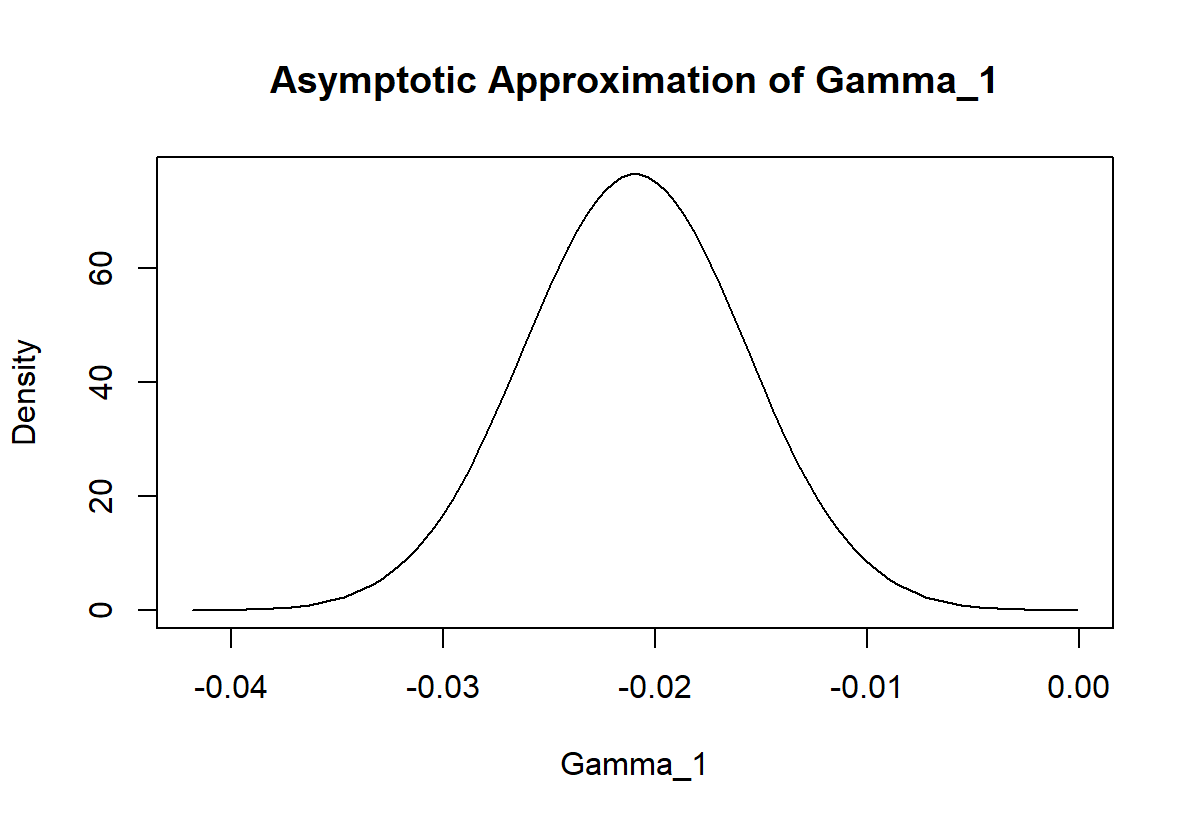
\includegraphics[width=0.5\linewidth]{i.png}
        \caption{Comparison of Bootstrap and Asymptotic Distributions of Gamma\_1}
        \label{fig:i}
    \end{figure}

    \begin{lstlisting}[language=R]
phi_age_60 <- dnorm(sum(x_age_60 * beta_hat))
phi_age_30 <- dnorm(sum(x_age_30 * beta_hat))
grad_g <- phi_age_60 * x_age_60 - phi_age_30 * x_age_30

print(grad_g)

# Compute asymptotic variance
var_gamma_1 <- t(grad_g) %*% V_hat %*% grad_g / nrow(dat_1000)
gamma_1_sd <- sqrt(var_gamma_1)

simulated_gamma <- rnorm(1000, mean = gamma_1, sd = gamma_1_sd)

bootstrap_data2 <- data.frame(Value = gamma_1_bootstrap, Distribution = "Bootstrap")
simulated_data2 <- data.frame(Value = simulated_gamma, Distribution = "Asymptotic")

# Combine data
combined_data2 <- rbind(bootstrap_data2, simulated_data2)

# Create the plot
ggplot(combined_data2, aes(x = Value, fill = Distribution)) +
  geom_histogram(aes(y = ..density..), bins = 20, position = "identity", alpha = 0.7, color = "black") +
  scale_fill_manual(values = c("Bootstrap" = "grey", "Asymptotic" = "orange")) +
  labs(title = "Comparison of Bootstrap and Asymptotic Distributions of Gamma_1",
       x = "Gamma_1 Estimation", y = "Density") +
  theme_minimal() +
  theme(plot.title = element_text(hjust = 0.5, size = 16),
        legend.title = element_blank(),
        legend.position = "topright",
        axis.title = element_text(size = 14),
        axis.text = element_text(size = 12)) +
  guides(fill = guide_legend(reverse = TRUE))        
    \end{lstlisting}
\end{autosolution}

\begin{autosolution}
    \

    We test
    \[
    H_0: \gamma_1(\beta)=0 \quad \text{vs.} \quad H_1: \gamma_1(\beta)\neq 0.
    \]
    Under the asymptotic approximation,
    \[
    \gamma_1(\hat{\beta}) \approx N\left(\gamma_1(\beta_0), \frac{1}{n}\hat{V}\right),
    \]
    where
    \[
    \hat{V} = \nabla_\beta \gamma_1(\hat{\beta})' \hat{H}^{-1} \nabla_\beta \gamma_1(\hat{\beta}).
    \]
    The t-statistic is:
    \[
    t = \frac{\gamma_1(\hat{\beta})}{\sqrt{\hat{V}/n}}.
    \]
    Empirically, $t \approx -0.68$.
    
    A 95\% confidence interval for $\gamma_1(\beta)$ is:
    \[
    \left[\gamma_1(\hat{\beta}) - 1.96 \sqrt{\frac{\hat{V}}{n}}, \gamma_1(\hat{\beta}) + 1.96 \sqrt{\frac{\hat{V}}{n}}\right].
    \]

    Empirically, the 95\% Confidence Interval for $\gamma_1(\beta)$ is: -0.0815 to 0.0396, covering 0. 
    
    So, we conclude that the expected probabilities of cash payment for a 30 year-old
    and a 60 year-old male buying clothes for 500 TRY are not significantly different.
    % \textbf{Graphical Analysis and Econometric Interpretation:}
    % \begin{itemize}
    %     \item The bootstrap histograms of the coefficient on age, $\gamma_1(\hat{\beta})$, and $\gamma_2(\hat{\beta})$ all resemble roughly normal shapes, centered near their estimated values. This supports the use of normal approximations.
    %     \item The asymptotic approximations (shown by smooth curves on histograms) align reasonably with the bootstrap distributions, suggesting that for $n=1000$, the asymptotic theory is not grossly inaccurate.
    %     \item The negative partial effects of age, though small in magnitude, show that older individuals might be slightly less likely to pay in cash. However, statistical tests indicate this difference is not significant at conventional levels.
    %     \item Category-specific differences matter, as seen from the significance of some category dummies. Clothes/Shoes, for example, differ in their propensity of cash usage compared to the base category.
    % \end{itemize}

    \begin{lstlisting}[language=R]
t_statistic <- gamma_1 / gamma_1_sd
critical_value <- qnorm(0.975)  # 1.96 for 95% confidence

if (abs(t_statistic) > critical_value) {
  conclusion <- "Reject the null hypothesis."
} else {
  conclusion <- "Fail to reject the null hypothesis."
}

print(paste("t-statistic:", round(t_statistic, 2)))
print(paste("Conclusion:", conclusion))

lower_bound <- gamma_1 - critical_value * gamma_1_sd
upper_bound <- gamma_1 + critical_value * gamma_1_sd

print(paste("95% Confidence Interval for gamma_1:", round(lower_bound, 4), "to", round(upper_bound, 4)))    
    \end{lstlisting}
\end{autosolution}

\end{document}